% Cap�tulo 3
\chapter{Implementação}

Este capítulo descreve as etapas das implementações do método em camadas e do método de Fridrich. Antes, é essencial definir alguns conceitos
e nomenclatura.

\section{Representação}

Para representar as faces do cubo de Rubik é utilizado o conceito de matrizes. Tendo em vista que o cubo é composto por seis faces, foram criadas seis matrizes do tipo inteiro, cada uma com três linhas e três colunas.


As cores do cubo são simbolizadas por um número inteiro e cada face é representada por uma cor, conforme mostrado na Tabela 4. A Figura \ref{fig:cuboresolvido} apresenta a visualização do cubo resolvido.



\begin{table}[!htb]   
    \textsf{\caption{Representação das faces do cubo de Rubik}}
    \centering
    \medskip
   
    \begin{tabular}{c|c|c}  
        \hline
        \textbf{Face} & 
        \textbf{Cor} &
        \textbf{Número} \\
        \hline
        D & Branco & 1  \\
        \hline
        U & Amarelo & 2  \\
        \hline
        F & Verde & 3  \\
        \hline
        R & Laranja & 4  \\
        \hline
        B & Azul & 5  \\
        \hline
        L & Vermelho & 6 \\
        \hline
        
    \end{tabular}
    \label{table:tabb}
\end{table}



\begin{figure}[!htb]
    \centering
    {
        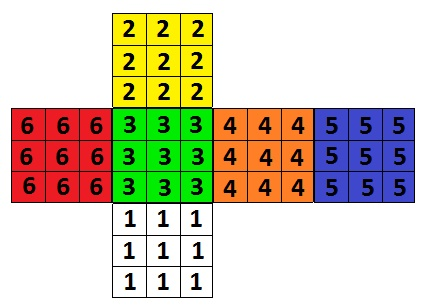
\includegraphics[height=5cm]{imagens/numerado.jpg}
        \label{figFront}
    }
    
\caption{Representação do cubo de Rubik}
\label{fig:cuboresolvido}
\legend{Fonte: Elaborado pelo autor (2017)}
\end{figure}


\section{Método em camadas}


O método em camadas, também conhecido como o método dos sete passos ou método básico, é simples e muito utilizado por quem tem interesse em aprender a solucionar o cubo de Rubik. Como o próprio nome sugere, essa solução consiste em resolver o cubo camada por camada, utilizando apenas sete passos.

\begin{itemize}
    \item Passo 1: fazer a cruz na face D;
    \item Passo 2: posicionar as peças de quina da primeira camada;
    \item Passo 3: posicionar as peças de meio da segunda camada;
    \item Passo 4: fazer a cruz na face U;
    \item Passo 5: orientar as peças de quina;
    \item Passo 6: permutar as peças de quina;
    \item Passo 7: permutar as peças de meio.    
\end{itemize}




\subsection{Modelo}

Para implementar o algoritmo em camadas foi utilizado a linguagem de programação Java. Para representar o cubo mágico e suas respectivas faces, utilizamos o conceito de classes. Os principais métodos da classe {\tt Face} são mostrados na Figura \ref{fig:figInterfaceFace}.

\begin{figure}[!htb]
    \centering
    {
        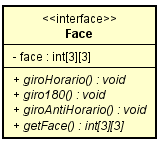
\includegraphics[height=3cm]{imagens/InterfaceFace.png}
        \label{figFront}
    }
    
\caption{Métodos e atributos da classe Face}
\label{fig:figInterfaceFace}
\legend{Fonte: Elaborado pelo autor (2017)}
\end{figure}


Essa classe contém uma matriz que representa a face do cubo mágico, assim como um método de acesso que retorna o atributo, chamado de {\tt getFace}. Existem outros três métodos que correspondem aos movimentos básicos que toda face do cubo pode realizar: {\tt giroHorario}, {\tt giro180} e {\tt giroAntiHorario}. O objetivo deles é modificar as peças de meio e as quinas, conforme os movimentos realizados no cubo.  


Já na classe {\tt Cubo} estão presentes seis atributos do tipo Face e três métodos para cada face, cada um representando os giros que as faces podem realizar. Por exemplo, para a face F foi implementado os seguintes métodos: {\tt giroF} (giro de 90º no sentido horário, ou simplesmente F), {\tt giroF2} (giro de 180º, ou F2) e {\tt giroFAntiHorario} (giro de 90º no sentido anti-horário, ou F’). Além deles, existem outros sete métodos que representam cada passo do algoritmo em camadas. Os métodos e atributos da classe Cubo são mostrados na Figura \ref{fig:figInterfaceCubo}.
\begin{figure}[!htb]
    \centering
    {
        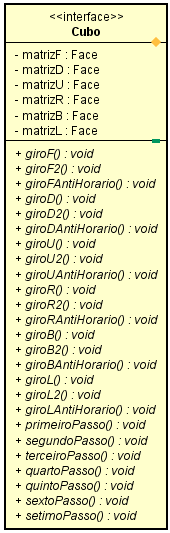
\includegraphics[height=10cm]{imagens/Cubo.png}
        \label{figFront}
    }
    
\caption{Métodos e atributos da classe Cubo}
\label{fig:figInterfaceCubo}
\legend{Fonte: Elaborado pelo autor (2017)}
\end{figure}

\subsection{Algoritmos}

O passo inicial dessa técnica é fazer uma cruz na face D. Para isso, é necessário analisar todas as posições onde poderão ser encontradas as peças de meio de cor branca. Após essa análise, os métodos necessários para reposicionar das peças são invocados. A seguir é mostrado um trecho de código em Java que ilustra o primeiro passo do algoritmo em camadas.

\begin{figure}[!htb]
\begin{lstlisting}
public void primeiroPasso(){
    // Reposicionando a peca DF 
    if (matrizD[1][2] == 1 && matrizR[2][1] == 3) {
         giroDAntiHorario();
    } else if (matrizD[2][1] == 1 && matrizB[2][1] == 3) {
        giroD2();
    } else if (matrizD[1][0] == 1 && matrizL[2][1] == 3) {
        giroD();
    }
    ...
}
\end{lstlisting}
\caption{Código parcial do primeiro passo}
\label{fig:figcoasasqd1}
\end{figure}

No método acima, foram mapeadas todas as 23 possibilidades para reposicionar a peça DF no seu local correto. Para a peça DL foram 21 possibilidades, para a DB foram 19 e para DR foram 17. O objetivo da primeira etapa é chegar à configuração ilustrada na Figura \ref{fig:primeiroPasso}.

\begin{figure}[!htb]
    \centering
    {
        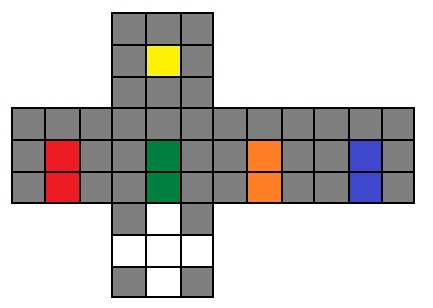
\includegraphics[height=5cm]{imagens/primeiroPasso.jpg}
        \label{figFront}
    }
    
\caption{Ilustração do primeiro passo}
\label{fig:primeiroPasso}
\legend{Fonte: Elaborado pelo autor (2017)}
\end{figure}


O passo seguinte é responsável por localizar as peças da face D em todas as seis matrizes do cubo para finalizar a primeira camada. Como a cruz já está completa, as peças que faltam são as quinas de cor branca, assim, é preciso mapear todas as posições em que possam ser encontradas peças de quina. 

Para fazer a orientação da peça DFR foi necessário analisar 23 possibilidades, já no caso da DFL foram analisadas 20 posições possíveis. Para orientar as peças DLB e DRB foi preciso codificar, respectivamente, 17 e 14 possibilidades de localização que essas peças poderiam estar situadas. Um pequeno trecho do código do segundo passo pode ser observado na Figura \ref{fig:figcodsds1}. 


\begin{figure}[!htb]
\begin{lstlisting}
public void segundoPasso(){
   // Reposicionando a peca DFR
   if (matrizD[0][0] == 1 && matrizF[2][0] == 4 && matrizL[2][2] == 3) {
      giroLAntiHorario();
      giroUAntiHorario();
      giroL();
      giroR();
      giroU();
      giroRAntiHorario();
   }
   ...
}
\end{lstlisting}
\caption{Código parcial do segundo passo}
\label{fig:figcodsds1}
\end{figure}

Ao finalizar este passo, todas as peças da base do cubo estarão  corretamente posicionadas. Além disso, as peças das faces laterais devem estar posicionadas em relação à cor dos centros de suas respectivas faces, como mostra a Figura \ref{fig:segundoPasso}.


\begin{figure}[!htb]
    \centering
    {
        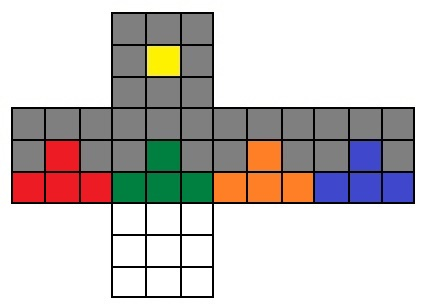
\includegraphics[height=5cm]{imagens/segundopasso.jpg}
        \label{figFront}
    }
    
\caption{Ilustração do segundo passo}
\label{fig:segundoPasso}
\legend{Fonte: Elaborado pelo autor (2017)}
\end{figure}

O mesmo mapeamento nas matrizes é feito para solucionar a segunda camada e concluir a terceira etapa. Dessa vez procurando por peças de meio que correspondem às faces F, R, B e L. No caso da peça FR, foi necessário implementar 15 possibilidades. Para orientar a peça FL foi preciso analisar 13 casos para poder reposicioná-la. Já para as peças BL e BR foi preciso analisar 11 e 9 casos, respectivamente. A Figura \ref{fig:figcoood1} mostra um trecho da implementação do terceiro passo.

Essa etapa gera uma quantidade maior de movimentos do que os passos anteriores, visto que, para orientar as peças de meio da segunda camada, é necessário deslocar as peças que já estavam na sua posição correta e reposicioná-las novamente. É interessante notar que nessa técnica o mesmo algoritmo é aplicado no máximo quatro vezes, uma vez que as peças FR, FL, BL e BR são posicionadas uma de cada vez. 



\begin{figure}[!htb]
\begin{lstlisting}
public void terceiroPasso(){
   // Reposionando a peca FR
   if (matrizF[0][1] == 3 && matrizU[2][1] == 4) {
      giroU();
      giroR();
      giroUAntiHorario();
      giroRAntiHorario();
      giroUAntiHorario();
      giroFAntiHorario();
      giroU();
      giroF();
   }
   ...
}
\end{lstlisting}
\caption{Código parcial do terceiro passo}
\label{fig:figcoood1}
\end{figure}


A Figura \ref{fig:terceiroPasso} ilustra o estado do cubo mágico após a execução do método que representa a terceira etapa.

\begin{figure}[!htb]
    \centering
    {
        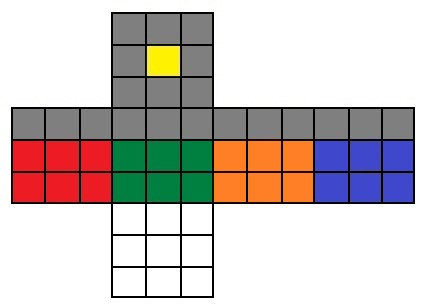
\includegraphics[height=5cm]{imagens/terceiropasso.jpg}
        \label{figFront}
    }
    
\caption{Ilustração do terceiro passo}
\label{fig:terceiroPasso}
\legend{Fonte: Elaborado pelo autor (2017)}
\end{figure}


Com a primeira e segunda camada concluídas, resta apenas a última camada. Para solucioná-la, é necessário executar os quatro últimos passos. A quarta etapa tem o objetivo de posicionar as peças de meio da face U de maneira que forme a figura de uma cruz.

O mapeamento é realizado através da análise das peças que não estão na sua posição correta e das peças que estão posicionadas corretamente, mas invertidas. Para concluir essa etapa são analisadas 7 possibilidades de localização das peças de meio. A Figura \ref{fig:figcodds1} mostra um trecho do código do método que resolve o quarto passo do algoritmo.



Vale destacar que, nessa etapa, diferentemente da cruz feita no primeiro passo, não importa se as peças estão orientadas, mas apenas se elas estão posicionadas de modo a forma uma cruz. A Figura \ref{fig:quartoPasso} ilusta o objetivo do quarto passo. 

\begin{figure}[!htb]
\begin{lstlisting}
public void quartoPasso(){
    if(matrizF[0][1] != 2 && matrizU[2][1] != 2 && matrizU[1][0] == 2 && matrizU[1][2] == 2){
        giroF();
        giroR();
        giroU(); 
        giroRAntiHorario();
        giroUAntiHorario();
        giroFAntiHorario();
   }
   ...
}
\end{lstlisting}\caption{Código parcial do quarto passo}
\label{fig:figcodds1}
\end{figure}




\begin{figure}[!htb]
    \centering
    {
        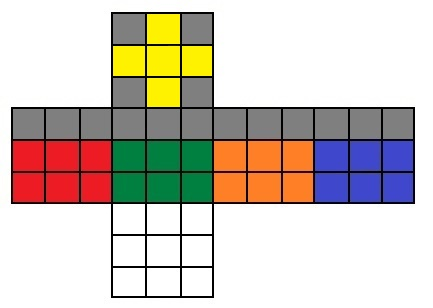
\includegraphics[height=5cm]{imagens/quartopasso.jpg}
        \label{figFront}
    }
    
\caption{Ilustração do quarto passo}
\label{fig:quartoPasso}
\legend{Fonte: Elaborado pelo autor (2017)}
\end{figure}


O quinto passo finaliza a face U do cubo por completo, posicionando todas as peças de quina para o topo. Nesse passo, não importa se as peças estão orientadas, o importante é que elas estejam posicionadas de modo que a face U contenha apenas peças de cor amarela.



Há 7 possibilidades para solucionar essa etapa. Em todos os casos será executado apenas um algoritmo, popularmente chamado de Sune, variando apenas a quantidade de vezes que ele deverá ser aplicado, dependendo, em todos os casos, do posicionamento das peças. A Figura \ref{fig:figcodpasso5} mostra um trecho de código que corresponde ao método responsável por executar o quinto passo. O código mostrado na imagem é a implementação do primeiro caso.


\begin{figure}[!htb]
\begin{lstlisting}
public void quintoPasso(){
    // CASO 1
    if (matrizU[2][0] == 2 && matrizF[0][2] == 2 && matrizR[0][2] == 2 && matrizB[0][0] == 2) {
        giroR();
        giroU();
        giroRAntiHorario();
        giroU();
        giroR();
        giroU2();
        giroRAntiHorario();
   }
   ...
}
\end{lstlisting}
\caption{Código parcial do quinto passo}
\label{fig:figcodpasso5}
\end{figure}


O objetivo do quinto passo é ilustrado na Figura \ref{fig:quintoPasso}. Seu objetivo é apenas completar a face U com peças da cor amarela, desconsiderando as peças da terceira camada das faces F, R, L e B.  


\begin{figure}[!htb]
    \centering
    {
        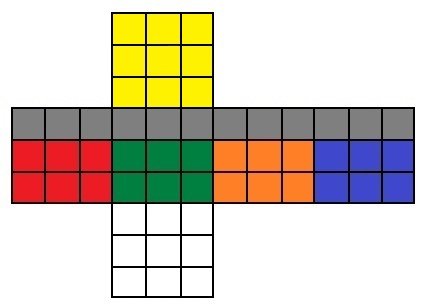
\includegraphics[height=5cm]{imagens/quintopasso.jpg}
        \label{figFront}
    }
    
\caption{Ilustração do quinto passo}
\label{fig:quintoPasso}
\legend{Fonte: Elaborado pelo autor (2017)}
\end{figure}


A finalidade do sexto passo é permutar as quatro peças de quina da última camada. O algoritmo faz o mapeamento para localizar a face que tem duas quinas de mesma cor, ou seja, verifica qual das faces F, R, L e B tem as peças de quina com cores iguais. No caso de não haver face com quinas iguais, aplica-se o algoritmo e em seguida o mapeamento é realizado mais uma vez. Depois de identificada a face que satisfaz essa condição, a mesma sequência de movimentos é aplicada mais uma vez. 

A Figura \ref{fig:figfsfsdxx} mostra um pequeno trecho de código que implementa esse passo. Pode-se observar que a estrutura condicional verifica se os valores das posições 0,0 e 0,2 da {\tt matrizB} (face B) são iguais, isto é, se as peças que estão nessas posições possuem a mesma cor. Essa mesma verificação é realizada nas peças de quina das matrizes que representam as faces F, R e L.




\begin{figure}[!htb]
\begin{lstlisting}
public void sextoPasso(){
    if (matrizB[0][0] == matrizB[0][2]) {
        giroRAntiHorario();
        giroF();
        giroRAntiHorario();
        giroB2();
        giroR();
        giroFAntiHorario();
        giroRAntiHorario();
        giroB2();
        giroR2();
   }
   ...
}
\end{lstlisting}
\caption{Código parcial do sexto passo}
\label{fig:figfsfsdxx}
\end{figure}


O resultado do sexto passo é ilustrado na Figura \ref{fig:sextopasso}.

\begin{figure}[!htb]
    \centering
    {
        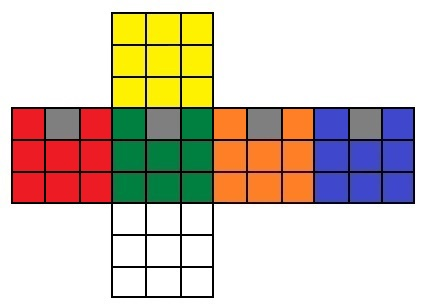
\includegraphics[height=5cm]{imagens/sextopasso.jpg}
        \label{figFront}
    }
    
\caption{Ilustração do sexto passo}
\label{fig:sextopasso}
\legend{Fonte: Elaborado pelo autor (2017)}
\end{figure}


O sétimo e último passo é responsável pela permutação das peças de meio da última camada. O algoritmo busca pelo lado do cubo que está totalmente resolvido, ou seja, verifica qual das faces F, R, L e B está totalmente solucionada. Geralmente os passos são executados apenas uma vez. No entanto, se nenhuma dessas faces estiverem completamente montadas, os passos são executados duas vezes. 


A Figura \ref{fig:fiwwwwwww} mostra uma parte do código utilizado na implementação do algoritmo. Como a primeira e segunda camada já estão solucionadas, o algoritmo verifica apenas as peças de meio e de quina. Espera-se que ao fim dessa etapa o cubo de Rubik esteja solucionado, como mostra a Figura \ref{fig:setimopassox}.

\begin{figure}[!htb]
\begin{lstlisting}
public void setimoPasso(){
    if ((matrizB[0][0] == matrizB[0][1]) && (matrizB[0][1] == matrizB[0][2])) {
        giroF2();
        giroU();
        giroRAntiHorario();
        giroL();
        giroF2();
        giroR();
        giroLAntiHorario();
        giroU();
        giroF2();   
    }
    ...
}
\end{lstlisting}
\caption{Código parcial do sétimo passo}
\label{fig:fiwwwwwww}
\end{figure}




\begin{figure}[!htb]
    \centering
    {
        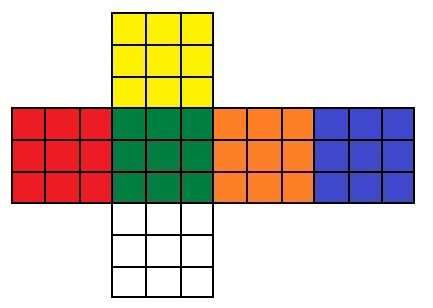
\includegraphics[height=5cm]{imagens/setimopasso.jpg}
        \label{figFront}
    }
    
\caption{Ilustração do sétimo passo: cubo solucionado}
\label{fig:setimopassox}
\legend{Fonte: Elaborado pelo autor (2017)}
\end{figure}

Ao executar os métodos, o resultado é uma sequência de movimentos que representam a solução gerada pelo método de camadas tradicional.


\section{Fridrich}



A implementação do algoritmo de Fridrich utiliza o mesmo conceito que a técnica anterior. A classe Face continua a mesma, com os mesmos métodos e atributos, como ilustrado na imagem \ref{fig:figInterfaceFace}. Na classe Cubo, no entanto, não existe mais os métodos que executavam os seis últimos passos do tradicional método em camadas. Ao invés disso, foram gerados outros métodos que representam os passos do novo algoritmo. Os novos métodos implementados são: F2L, OLL e PLL. 


Como a primeira etapa do método de Fridrich é exatamente a mesma do método de camadas, o código implementado é o mesmo da Figura \ref{fig:figcoasasqd1}.  

O objetivo do segundo passo é solucionar as duas primeiras camadas simultaneamente. O conjunto de passos que solucionam essas duas camadas é chamado de F2L. A imagem \ref{fig:fridrich2} mostra um trecho de código da implementação desse método. O algoritmo é extenso, possui exatamente 41 casos e, para cada caso, há 16 possibilidades de posicionamento das peças. 


\begin{figure}[!htb]
\begin{lstlisting}
public void f2l(){
    if (matrizF[0][2] == 1 && matrizU[2][2] == 3 && matrizR[0][0] == 4 && matrizU[1][2] == 3 && matrizR[0][1] == 4) {
        giroU();
        giroR();
        giroUAntiHorario();
        giroRAntiHorario();
    }
    ...
}
\end{lstlisting}
\caption{Código parcial do F2L}
\label{fig:fridrich2}
\end{figure}

A ordem de execução dos casos depende da quantidade de movimentos que cada um gera. Assim, de acordo com a Tabela 1 (Capítulo 2), os primeiros casos a serem analisados são os do grupo Easy Case, pois resultam em 3 ou 4 movimentos, e o último caso pertence ao grupo Weird, visto que gera até 13 movimentos. O resultado esperado ao fim da execução do método é ilustrado na Figura \ref{fig:terceiroPasso}.


No próximo passo, chamado de OLL, a finalidade do algoritmo é posicionar todas as peças amarelas na face U, independentemente de estarem orientadas. 

\begin{figure}[!htb]
\begin{lstlisting}
public void oll(){
    if (matrizU[0][1] == 2 && matrizU[1][0] == 2 && matrizU[1][2] == 2 && matrizU[2][1] == 2) {
        if (matrizU[0][2] == 2 && matrizR[0][0] == 2 && matrizF[0][0] == 2 && matrizL[0][0] == 2) {
            giroR();
            giroU2();
            giroRAntiHorario();
            giroUAntiHorario();
            giroR();
            giroUAntiHorario();
            giroRAntiHorario();
        }
        ...
    }
    ...
}
\end{lstlisting}
\caption{Código parcial do OLL}
\label{fig:fridrich3}
\end{figure}

Na implementação, as matrizes {\tt matrizU}, {\tt matrizF}, {\tt matrizR}, {\tt matrizL} e {\tt matrizB} são analisadas com o propósito de verificar se em alguma de suas posições existe o valor 2. Todos os 57 casos são foram implementados. A imagem \ref{fig:fridrich3} mostra um pequeno trecho do código. 



O último algoritmo do método de Fridrich é o PLL, que faz a permutação de todas as peças da face U com o objetivo de finalizar a solução, é ilustrado na Figura \ref{fig:fridrich4}.




\begin{figure}[!htb]
\begin{lstlisting}
public void pll(){
    if ((matrizB[0][0] == matrizB[0][1] && matrizB[0][1] == matrizB[0][2]) && (matrizR[0][2] == matrizR[0][0] && matrizR[0][0] == matrizL[0][1]) && (matrizF[0][0] == matrizF[0][2] && matrizF[0][2] == matrizR[0][1]) && (matrizL[0][0] == matrizL[0][2] && matrizL[0][2] == matrizF[0][1])) {
        giroR2();
        giroU();
        giroR();
        giroU();
        giroRAntiHorario();
        giroUAntiHorario();
        giroRAntiHorario();
        giroUAntiHorario();
        giroRAntiHorario();
        giroU();
        giroRAntiHorario();
    }
    ...
}
\end{lstlisting}
\caption{Código parcial do PLL}
\label{fig:fridrich4}
\end{figure}

Esse algoritmo analisa as matrizes que representam as faces U, F, L, R e B para realizar os 21 casos. Assim como nos passos anteriores, a ordem de execução dos casos depende do total de giros realizados, como mostra a Tabela 3. Ao executar esse método, a solução é concluída.





